\noindent 
To guide the discussion of the proposed research we present an overview of the system architecture that we will design and build. 
The system will rely on processing-in-memory architecture, but appropriately adopted for matrix manipulations used in graph processing.   
Figure~\ref{fig:arch} present the overview of the architecture. 
The GAMA (graph acceleration through matrix abstraction) system consists of 16 tiles; and each tile, called the GAMA tile, consists of a GAMA core closely tied to four 8GB DiRAM4 dies. 
DiRAM4 is a die-stacked DRAM die from Tezzaron.
% (one of our service providers in this project). 
The unique aspect of DiRAM4 compared to other competing memories, such as high bandwidth memory (HBM), is that each DiRAM4 die supports more channels per die, but uses narrower channels than HBM. 
%Such a design is well suited for graph workloads that need memory-level parallelism to access multiple vertices concurrently. 
Such a design is well suited for graph workloads that need memory-level parallelism to efficiently access both random/sparse and sequential/dense data arrays concurrently. 
We will use 2.5D integration to connect a GAMA core die with four DiRAM4 dies, thereby supporting 4TB/s aggregate in-package bandwidth per tile.  
16 GAMA tiles are clustered together using 1TB/s inter-tile interconnects to form the full GAMA system. 

Each GAMA tile is built as an SMX2 form factor accelerator board that will be interfaced with an IBM OpenPower system through the Coherent Accelerator Processor Interface (CAPI);
Kim and Hwu have been working with IBM's OpenPower and CAPI teams for an IBM project, and IBM agreed to provide technical support for this project as well. % to showcase this  at the OpenPower Submmit.
%We will rely on the OpenPOWER mother board which provides OpenCAPI interface through SMX2 sockets.  
Traditionally IBM Power8 supported 8 DMI (differential memory interface) links  to connect to external memory. 
Recently IBM demonstrated ConTutto Card design for integrating an FPGA accelerator into P8 by plugging into one of the DMI links. 
We will be using the same approach to design a single GAMA tile card that will be integrated into a DMI link. 
Two IBM Power8 hosts will be used and each host will connect to eight GAMA tiles.  
IBM will be providing the services for enabling OpenCAPI interface on each GAM tile. 
IBM will also be building a custom board that is based on OpenPOWER design. 
The OpenPOWER mother board provides OpenCAPI interface through SMX2 sockets that will host the GAMA tiles. 
The board enables up to 16 SMX2 tiles connected either to OpenPOWER cores or among themselves. 
The GAMA  system is interfaced with the memory channel of a host CPU using the OpenCAPI providing up to 8 memory channels per GAMA system.

Although CAPI provides coherent memory interface to the accelerators, in this proposal the memory space associated with the GAMA system is a non-cacheable region to eliminate the need for managing cache coherence between caches of the host systems and GAMA tiles. 
%M - do we need the above sentence?
Each GAMA core consists of 32 MIMD-style corelets, each with three separate \emph{elastic} L1 caches. 
The elastic cache is a specialized cache organization that supports variable width cache lines to improve cache usage efficiency.  
As such the elastic L1 caches are architected to support both dense/sequential and sparse/random accesses.
Furthermore, all the corelets share a elastic spatial-temporal boosting eDRAM cache which acts as a shared L2 cache. 

Corelets support a reconfigurable execution pipeline that is designed for doing various matrix operations in an ASIC flow. 
For instance, a single fused floating-point multiply-accumulate operation across a sparse row and a sparse vector may be configured to find the single hop neighbors of a given vertex, which is typically one iteration of a breadth first search algorithm. 
%NAM: WHAT ARE THE OTHER OPERATIONS THAT YOU ENVISION? I AM NOT SURE IF MATRIX OPERATIONS HAVE MUCH OF ANYTHING ELSE.  

\begin{figure}
\center
%\vspace{-8ex}
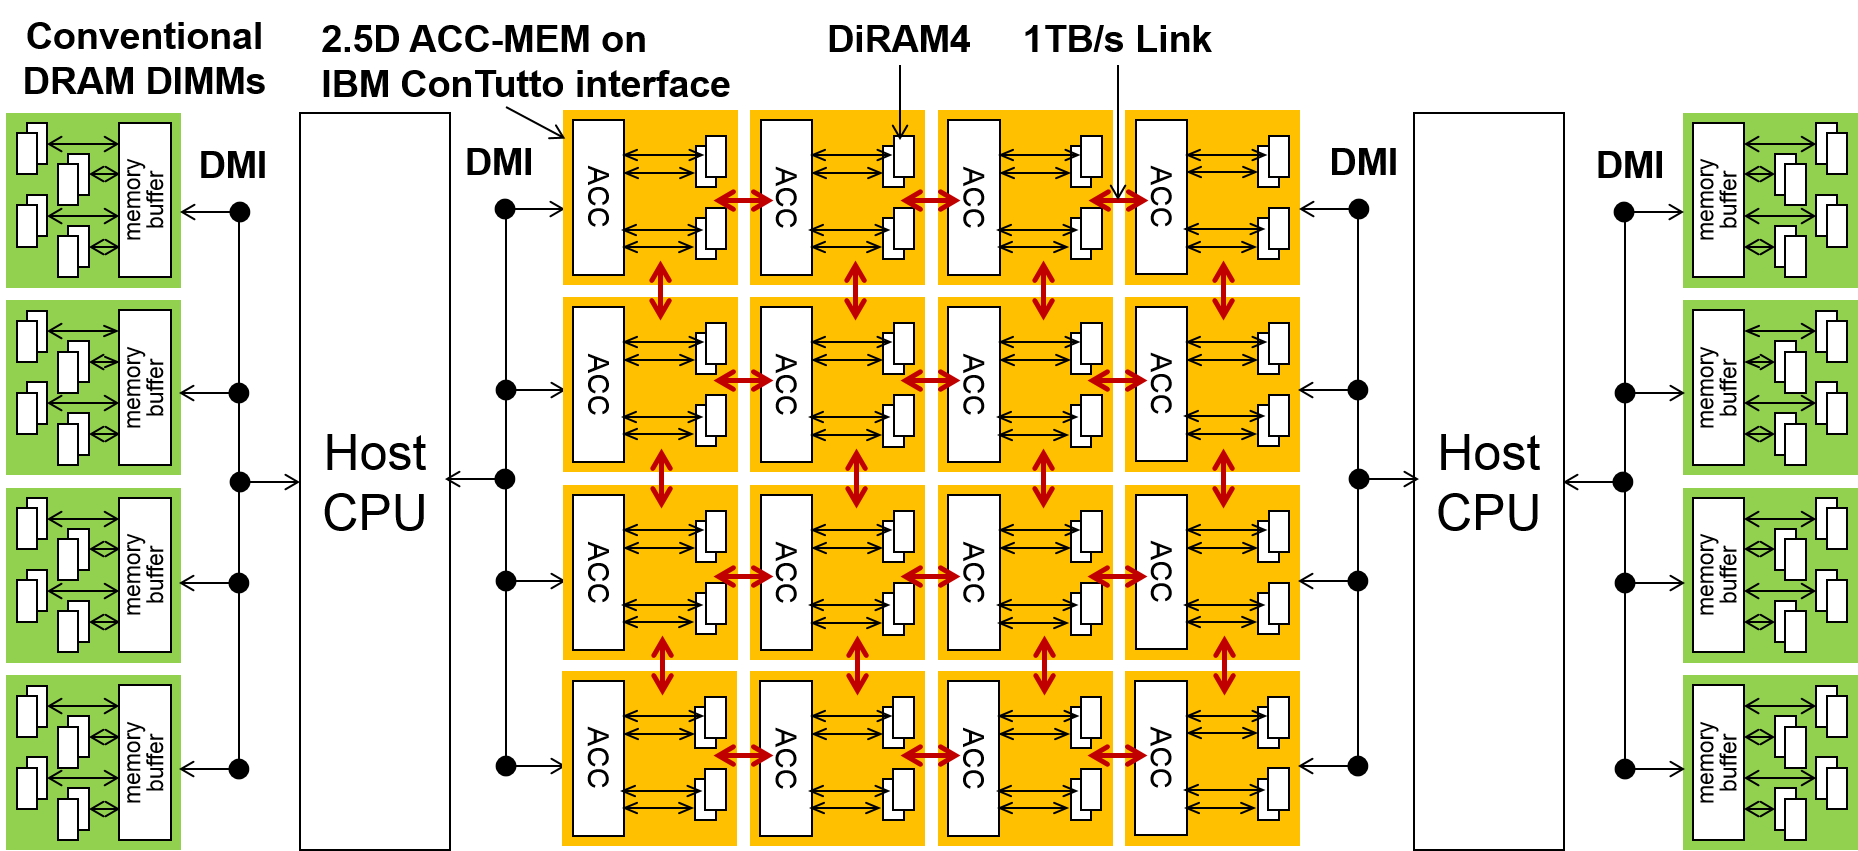
\includegraphics[width=1.0\linewidth]{fig/arch.png}
\caption{GAMA System Architecture}
\label{fig:arch}
\end{figure}
 


\begin{comment}

%the memory channel provides the highest bandwidth with the lowest latency amongst off-chip communication interfaces in contemporary computer systems.

 
 %Specifically,  a DiRAM4 die provides the same aggregate bandwidth as HBM2, but it provides 4X more channels than HBM2 where each channel supports only a quarter of the width of HBM2. We believe that DiRAM4 design is better suited for graph analytics where multiple accesses are made to random 


High bandwidth memory (HBM) and hybrid memory cube (HMC) used for recent PIM architectures can provide high bandwidth only for sequential, regular memory accesses. In contrast, graph analytics require efficient support for irregular and small granularity memory accesses. We tackle this problem by adopting a recent DiRAM4 3D Memory from Tezzaron and architecting on-chip caches and a custom memory controller to efficiently support small granularity irregular memory accesses. 
Specifically, DiRAM4 provides the same aggregate bandwidth as HBM2, but it provides 4$\times$ more (but narrower) channels than HBM2

.  The tiled architecture is built  

In this project, we envision to develop a PIM system depicted in Figure~\ref{fig:arch}. 
Overall, the system consists of a 16-node accelerator-memory (AM) cluster and IBM POWER8-based host systems.
An AM cluster is comprised of 16 nodes (packages) connected by our power-efficient high-bandwidth chip-to-chip links in a mesh style. 
One accelerator (ACC) and four 8GB DiRAM4 dies will constitute a PIM package with 4TB/s aggregate in-package bandwidth. 
%Our ACC die will integrate 16 ACCs with our custom eDRAM-based large shared and SRAM-based private on-chip cache, a 16$\times$16 crossbar, and a network interface (NI) to support chip-to-chip communications.

\begin{wrapfigure}{r}[0pt]{0.6\textwidth}
\center
%\vspace{-8ex}
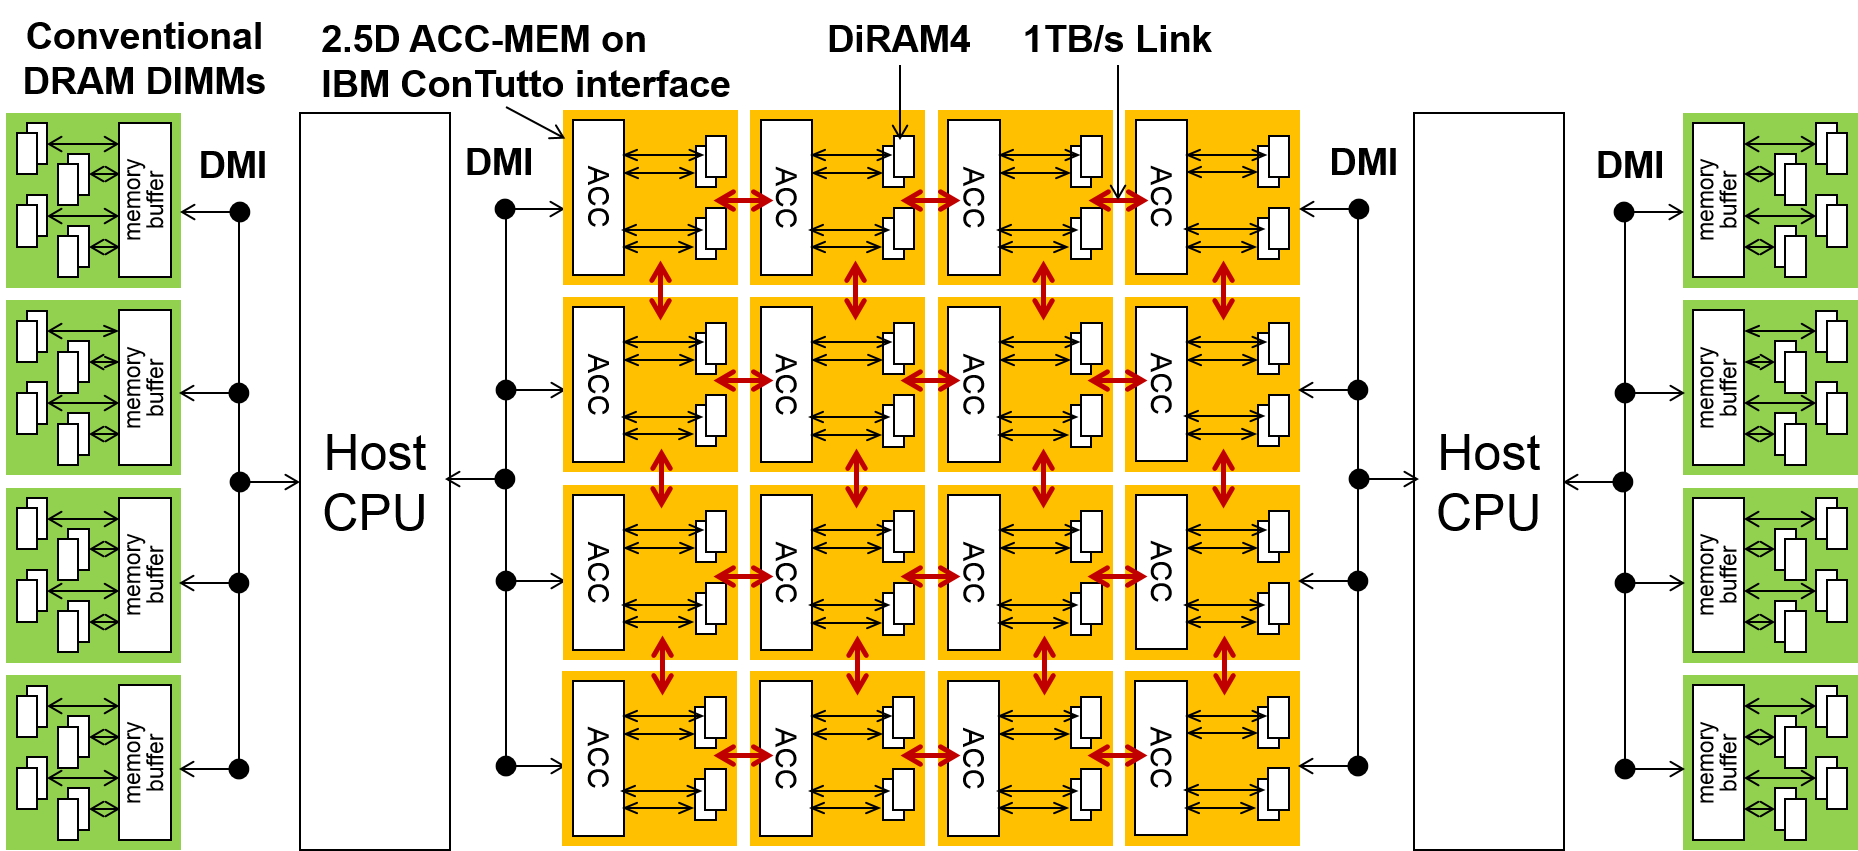
\includegraphics[width=1.0\linewidth]{./fig/arch.png}
\caption{The overall architecture of an Accelerator-Memory HIVE.}
\label{fig:arch}
\end{wrapfigure}

In the proposed PIM system, we propose to connect each AM packages to a memory channel of a host CPU providing 8 memory channels;
the memory channel provides the highest bandwidth with the lowest latency amongst off-chip communication interfaces in contemporary computer systems.
A IBM's ConTutto facilitates the interface between an AM package and the IBM's proprietary memory interface (DMI).
The memory space associated with the AM cluster is a non-cacheable region to eliminate the need for managing cache coherence between caches of the host systems and the AM HIVE.
The host system allocates the memory space of the AM cluster as a sinlge, continuous, and large physical memory segment which is preferred by big-data applications~\footnote{}.
ACCs are memory-mapped to part of the non-cacheable regions (as other I/O devices).

% Some notes
% We need a custom POWER8 board
\end{comment}
